\subsection{Auswahl des Experimentes und physikalischer Hintergrund}
\label{sec-2-3}
Zuvor soll jedoch noch kurz auf die Auswahl des vorgestellten Versuches eingegangen werden.

\subsubsection{Auswahl des Experimentes}
\label{sec-2-3-1}
Das Experiment wurde neben den bereits erörterten Gründen und Motivationen auch aus technischen und praktischen Aspekten ausgewählt. Im Wesentlichen trugen dazu die folgenden Faktoren bei:
\begin{itemize}
	\setlength{\itemsep}{-1pt}
	\singlespacing
	\item Die notwendigen Materialien (Spule, Messgeräte, Simulationslösung) standen für diese Arbeit zur Verfügung.
	\item Das Magnetfeld der Spule hat keine erkennbaren Auswirkungen auf die HoloLens (das Gerät nutzt ein Magnetometer). Tests im Vorfeld mit Flussdichten von über 100 Mikrotesla zeigten keine wahrnehmbaren Auswirkungen auf das Tracking und die Stabilität von Hologrammen.
	\item Die gegebene Größe der Spule (R=15cm) eignet sich für das beschränkte Sichtfeld der HoloLens.
	\item Das Experiment enthält keine sich schnell bewegenden Elemente und ist bis auf den Kompass statisch, es erfordert außerdem keine besondere Schutzausrüstung
\end{itemize}

Diese Umstände begünstigen einen Einsatz der Brille für diesen konkreten Anwendungsfall und sind ggf. bei anderen Szenarien so nicht gegeben.

Helmholtz-Spulen werden in der Physik an verschiedenen Stellen verwendet und spielen auch in der Ausbildung von Schülern und Studenten eine wichtige Rolle. Unter anderem werden sie in Schülerversuchen genutzt, um experimentell die Stärke des Erdmagnetfeldes zu bestimmen. Im Folgenden sollen die physikalischen Hintergründe kurz eingeführt sowie der Versuchsaufbau und -Ablauf erläutert werden.

\subsubsection{Spulen und Magnetfelder}
\label{sec-2-3-2}
Ein Magnetfeld kann als dreidimensionales Vektorfeld aufgefasst werden. Die Stärke an einem Punkt lässt sich über den Feldstärkevektor $\boldsymbol{H}$ sowie die Flussdichte $\boldsymbol{B}$ angeben. Beide Größen hängen über eine Materialkonstante $\mu$ zusammen: $\boldsymbol{B} = \mu \cdot \boldsymbol{H}$.
\par
\noindent\hspace*{5mm}
Wird eine elektrische Leiterschleife von einem Strom durchflossen, so induziert diese ein Magnetfeld. Dieses Feld verläuft sowohl durch das Innere als auch durch die Umgebung der Spule. Die Stärke des Feldes hängt dabei von der Windungszahl und dem Durchmesser der Spule sowie der anliegenden Stromstärke ab.
Im Zentrum der Spule ist das Magnetfeld \textit{homogen}. Das bedeutet, es ist an allen Punkten im Raum gleich stark und gleich gerichtet. Außerhalb und am Rand der Spule hingegen ist das Feld \textit{inhomogen}, es erfüllt beide zuvor genannten Eigenschaften nicht.\\

\textit{Darstellungsformen von Magnetfeldern}\\
Zur Visualisierung von Magnetfeldern gibt es unterschiedliche Darstellungsmodelle. Im Bereich der Lehre haben sich davon vor allem zwei etabliert: Feldlinien und Vektoren. Beide stellen das Feld mit Richtung und Stärke im Raum dar, unterscheiden sich aber in der Art und Weise. Abbildung \ref{img:Magnetfeld-Helmholtzspule} zeigt eine gemeinsame Darstellung beider Ansätze für eine Helmholtz-Spule.\\

\begin{figure}[h!]
	\centering
	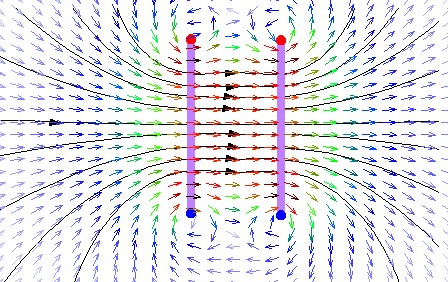
\includegraphics[width=0.65\textwidth]{images/papers/Magnetfeld-Helmholtzspule.jpg}
	\caption{Magnetfeld einer Helmholtz-Spule in der X-Z-Ebene. Der Betrag der Vektoren wurde hier statt der Länge über die Farbe kodiert. Die Feldlinien sind für einen mittigen Ausschnitt der Spule gezeichnet. Die Homogenität des Feldes im Inneren ist klar zu erkennen. Bildquelle: Wikipedia} %\footnote{\url{https://de.wikipedia.org/wiki/Helmholtz-Spule}}}
	\label{img:Magnetfeld-Helmholtzspule}
\end{figure}

\textit{Das Feldlinienmodell}\\
Die Feldliniendarstellung ist wohl die häufiger anzutreffende Darstellungsform. Hier werden kontinuierliche Linien genutzt, um den magnetischen Fluss darzustellen. Die Richtung des Feldstärkevektors an einem Punkt auf einer Feldlinie entspricht der Tangente an diesem Punkt. Die Stärke des Feldes wird meist proportional zur Dichte der Feldlinien dargestellt \cite{Kilian03}.\\

Diese Darstellung macht den Unterschied zwischen homogenen und inhomogenen Feldern besonders gut sichtbar, da bei einem homogenen Feld die Feldlinien parallel verlaufen, bei einem inhomogenen hingegen nicht. Außerdem ist die Darstellung über die Dichte der Feldlinien eng verbunden mit dem Konzept des magnetischen Flusses.\\

Allerdings bedeutet diese Darstellungsform auch, dass um so stärker das Feld ist, desto mehr Feldlinien auf gleichem Raum dargestellt werden müssen. Außerdem ist bei sich ändernden Feldern schwer zu erkennen, ob sich nur die Beträge der Feldstärkevektoren ändern, oder auch die Richtungen. Denn in beiden Fällen verändern sich Form und Abstand der Feldlinien.\\

\textit{Vektorfeld}\\
Im Gegensatz dazu wird in der Vektor-Darstellung das Feld über einzelne Vektoren repräsentiert. Dabei geben Richtung und Betrag eines Vektors den Feldstärkevektor des Magnetfeldes für genau einen Punkt an.\\
So lässt sich die Feldstärke an einem durch einen Vektor repräsentierten Punkt im Raum direkt ablesen. Wo ein Feld homogen ist lässt sich jedoch nur durch das Vergleichen von mehreren Vektoren in Länge und Richtung feststellen. Dieses Modell hat gegenüber dem Feldlinienmodell jedoch den Vorteil, dass mit zunehmender Feldstärke die Vektoren nur länger werden, ihre Anzahl jedoch gleich bleibt. Außerdem ist hier klar zu erkennen, ob bei einem sich ändernden Feld die Richtung der Vektoren konstant bleibt, oder nicht.

\subsubsection{Helmholtz-Spule}
\label{sec-2-3-3}
Bei einer Helmholtz-Spule handelt es sich im Prinzip um zum zwei zusammengeschaltete solcher Spulen. Dabei werden zwei identische Spulen nebeneinander aufgestellt und verbunden, sodass der Abstand genau dem Radius der Spulen entspricht. Abbildung \ref{img:Helmholtz} zeigt eine solche Helmholtz-Spule.\\

\begin{figure}[h!]
	\centering
	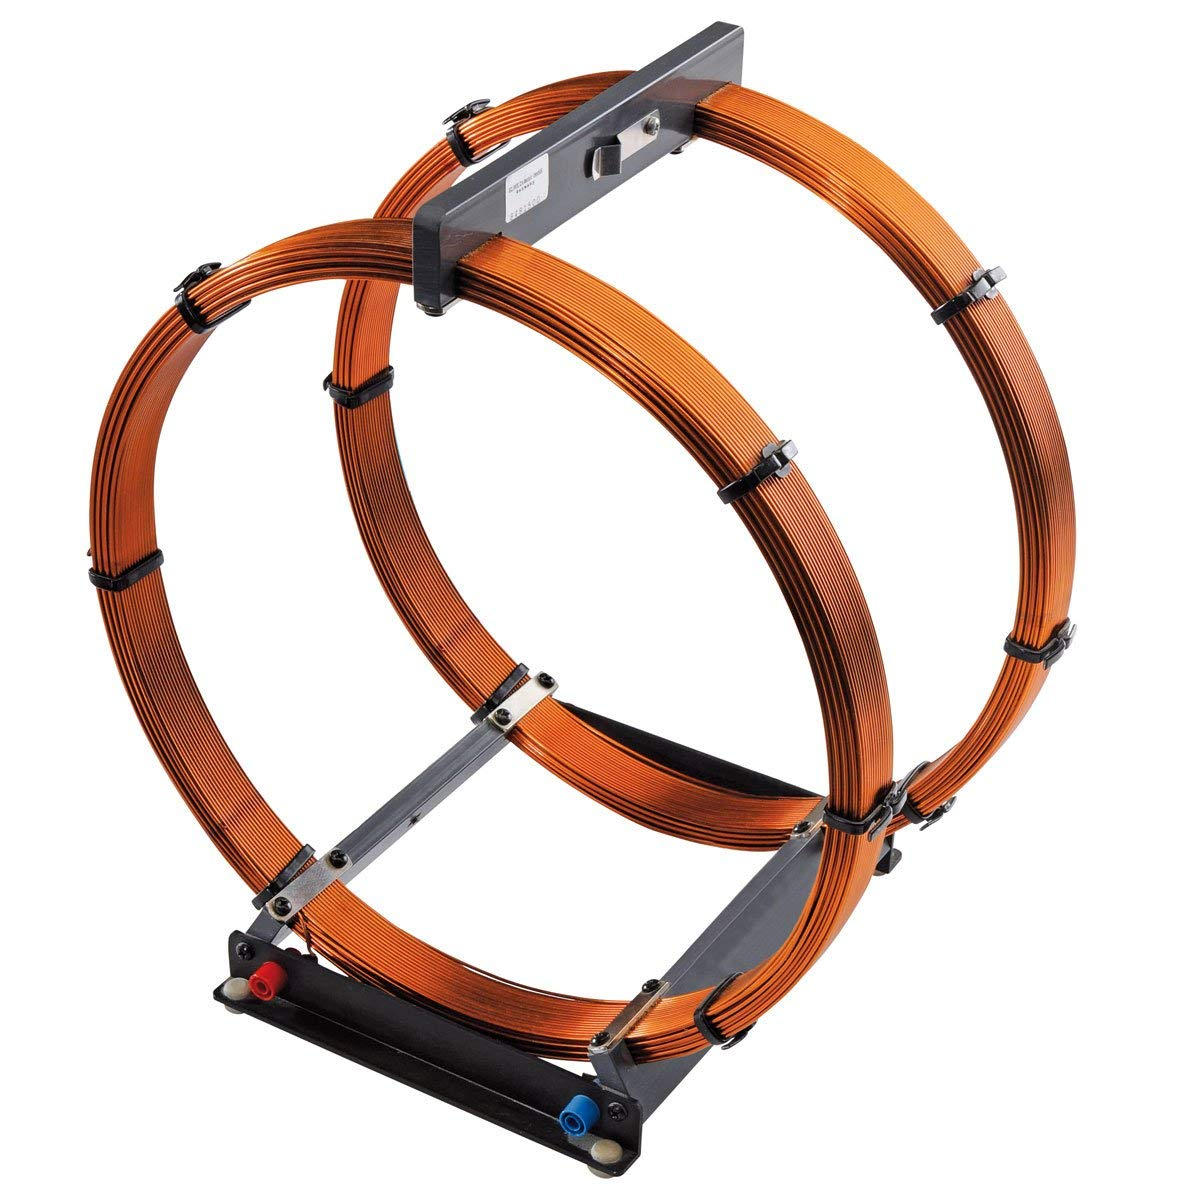
\includegraphics[width=0.45\textwidth]{images/papers/Helmholtz.jpg}
	\caption{HH Spule}
	\label{img:Helmholtz}
\end{figure}

Durch diese spezielle Eigenschaft des Aufbaus überlagern sich die beiden, durch die einzelnen Spulen entstehenden Magnetfelder genau so, dass im Raum zwischen den Spulen ebenfalls ein (nahezu) homogenes Magnetfeld entsteht. Abbildung \ref{img:Magnetfeld-Helmholtzspule} zeigt das Feld für die X-Z-Ebene in der Draufsicht von oben auf eine Helmholtz-Spule. Dabei ist zu erkennen, dass das Feld in weiten Teilen des durch die zwei Spulen aufgespannten Zylinders homogen ist. Lediglich am Rand und in unmittelbarer Nähe zu den Spulen wird das Feld zunehmend inhomogen. Detailliertere Informationen dazu finden sich beispielsweise in \cite{Demtroder13}.\\

Das Feld wird durch elliptische Integrale beschrieben, die nur numerisch zu lösen sind.
Die magnetische Flussdichte einer Helmholtz-Spule im Mittelpunkt zwischen den Spulen vereinfacht sich jedoch zu folgender Gleichung:
\begin{equation}
\label{eq:mfield}
B = \mu_{0} \cdot \frac{8 \cdot I \cdot N}{\sqrt{125} \cdot R}
\end{equation}

Dabei entspricht $I$ der Stromstärke, $N$ der Anzahl Windungen, $R$ dem Radius und $\mu_{0}$ der magnetischen Permeabilität. Die Stromstärke tritt dabei in der Feldgleichung als linearer Faktor auf. Änderungen an der Stromstärke rufen eine dazu proportionale Änderung der Feldstärke hervor. Außerdem bedeutet dieser Umstand, dass die Richtung des Feldstärkevektosrs nicht von der Stromstärke abhängt, sondern konstant bleibt.\\

\subsubsection{Versuchsaufbau und Ablauf}
\label{sec-2-3-4}
Ziel des Versuches ist die Bestimmung des Erdmagnetfeldes. Genauer bedeutet das die experimentelle Bestimmung von Richtung und magnetischer Flussdichte des Feldes. Die Richtung kann dabei allein über den Kompass bestimmt werden. Die Flussdichte wird aus der gemessenen Stromstärke ermittelt, bei der die Helmholtz-Spule ein gleich starkes, eigenes Magnetfeld erzeugt.\\

\textit{Aufbau}\\
Der Versuchsaufbau ist in Abbildung \ref{img:experiment-devices} dargestellt und besteht aus: 
\begin{itemize}
	\setlength{\itemsep}{-5pt}
	\item Einer Helmholtz-Spule mit fester Windungszahl und festem Radius
	\item Einem Kompass
	\item Einem in Reihe geschalteten Amperemeter
	\item Einem in Reihe geschalteten Widerstand	
	\item Einer angeschlossenen Spannungsquelle
\end{itemize}

\begin{figure}[h!]
	\centering
	\includegraphics[width=0.8\textwidth]{images/todo.jpg}
	\caption{Versuchsaufbau}
	\label{img:experiment-devices}
\end{figure}

\textit{Ablauf}\\
Der Versuch läuft in zwei Teilen ab. Zunächst wird die Ausrichtung des Erdmagnetfeldes bestimmt und im nächsten Schritt dann die Flussdichte. Der Ablauf lässt sich wie folgt zusammenfassen:
\begin{enumerate}
	\setlength{\itemsep}{-2pt}
	\item Kompassnadel nach Norden ausrichten lassen
	\item Helmholtz-Spule orthogonal zur Kompassnadel ausrichten
	\item Spannungsquelle einschalten und Spannung langsam erhöhen
	\item Spannung erhöhen, bis Kompassnadel um 45° ausgelenkt ist
	\item Stromstärke ablesen und in Gleichung \eqref{eq:mfield} einsetzen
\end{enumerate}

Durch dieses Vorgehen wird im zweiten Schritt durch die Spule ein Magnetfeld erzeugt, das orthogonal zu dem der Erde gerichtet ist. Beide Felder überlagern sich, so dass sie den Kompass genau dann gleichmäßig in beide Richtungen auslenken, wenn beide Felder gleich stark auf die Nadel wirken.

